%!TEX root=../paper.tex

\chapter{The Need for High-Performance and Energy-Efficient Computation in Mobile Web}
\label{sec:motivation}

This section quantitatively demonstrates the importance of \textit{computation}, among other components such as network and display, to mobile Web's performance and energy consumption. The observations discussed in this section directly motivate my research to focus on the computation layer of the mobile Web and to improve its performance and energy-efficiency.

The computation layer involves many mobile SoC components, such as CPU, GPU, and domain-specific accelerators. My work specifically focuses on the CPU for the following two reasons. First, CPU is the most heavily exercised computation component for Web applications because the Web runtime primarily targets CPUs. GPUs' usage, although providing critical performance benefits, is still limited to specific tasks such as rasterization and compositing~\cite{gpucompositor}. The key computations such as layout and JavaScript execution are still solely performed on general-purpose CPUs. Second, CPU serves as an incubator for future accelerators---we must first understand computation kernels' characteristics on CPUs before they can be accelerated. In fact, one of my dissertation contributions is the accelerator design of a key Web computation kernel based on its CPU execution behaviors.

In the rest of this section, I first show that the overall mobile Web performance depends increasingly on the computational capability of mobile CPUs, indicating the need for a high-performance computation~(\Sect{sec:motivation:perf}). I then show that mobile devices' power consumption is increasingly dominated by CPUs, calling for an energy-efficient computation~(\Sect{sec:motivation:energy}). Note that all the results presented in \Sect{sec:motivation:energy} are adapted from a recent research project~\cite{mobilecpu} that I collaborated on and contributed to.

\section{The Need for Compute Performance in Mobile Web}
\label{sec:motivation:perf}

Computation and network largely dictate the performance of mobile Web. Conventional wisdom suggests that mobile Web performance is primarily limited by the network latency. In this section, I quantify the impact of CPU and network performance by experimentally comparing how the webpage load time varies with different CPU and network performance on today's high-end smartphone Galaxy S5. I show that as cellular network technologies evolve over generations, mobile Web performance becomes sensitive to CPU performance.

\paragraph{Network Impact} Network performance is typically evaluated in two metrics: latency and bandwidth. Prior work has shown that in the mobile context, network latency---typically evaluated by round-trip time (RTT)---has a much more significant impact than network bandwidth~\cite{HPBN,browser-slow}. Therefore, we focus only on the latency aspect of network performance.

To study the impact of network latency of various cellular network generations, we host all the webpages on a Web server, into which we manually inject delay. We then use Wi-Fi on the smartphone to access the webpages. The delay injection lets us mimic a wide range of network latencies because Wi-Fi has significantly lower latency than the current 4G/LTE network. This methodology is well-established to control cellular network latency~\cite{browser-slow}.

\begin{figure}[t]
  \centering
  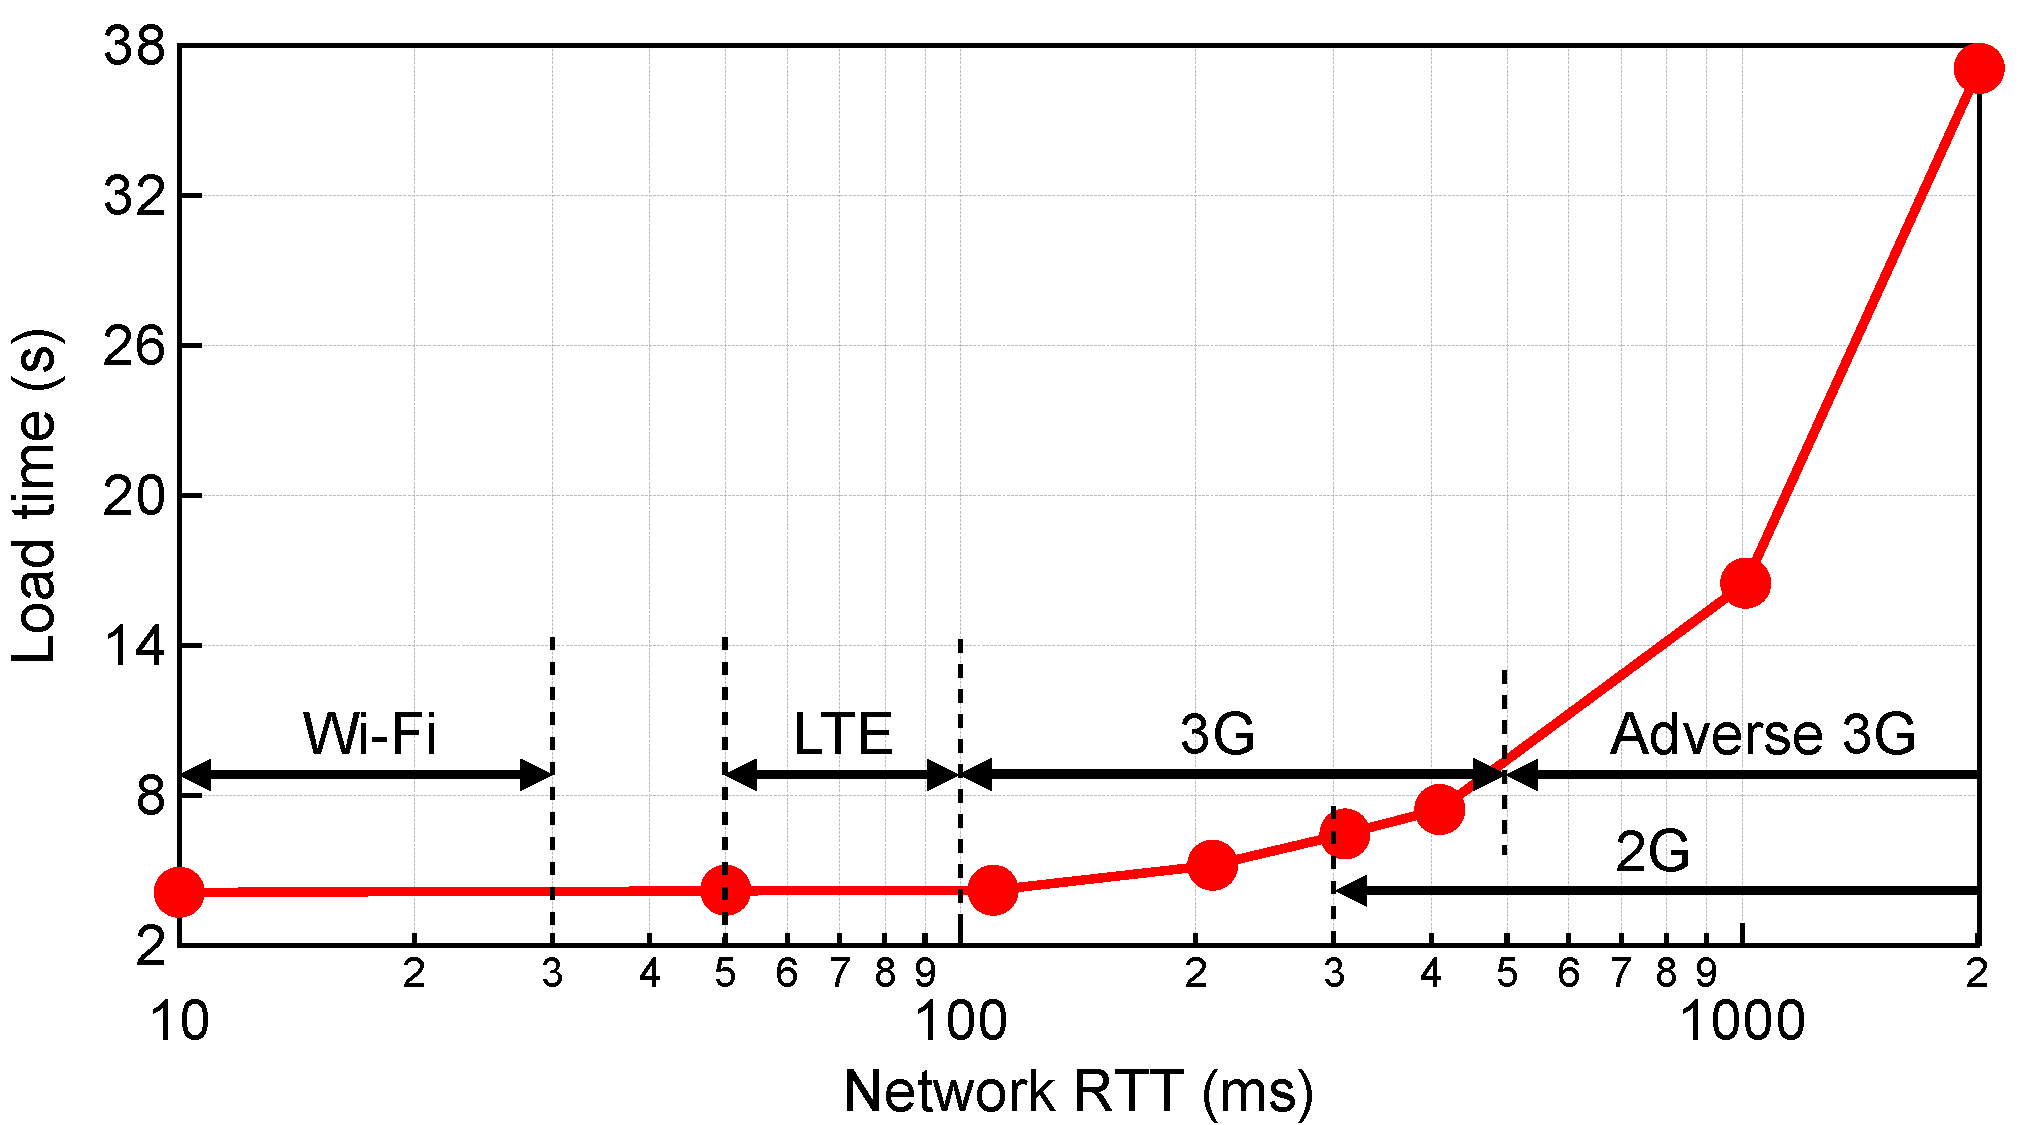
\includegraphics[trim=0 0 0 0, clip, width=.9\columnwidth]{network_bottleneck}
  \caption{Webpage load time with respect to changing network latency. Each marker corresponds to an RTT value. We also superimpose the round-trip time (RTT) range for different cellular technologies derived from both technical specifications as well as real measurements in the field~\cite{HPBN,carrier_measure}.}
  \label{fig:network_bottleneck}
\end{figure}

Holding the CPU performance at its peak, \Fig{fig:network_bottleneck} shows the webpage load time with respect to different network latencies. We superimpose the figure with different mobile network technologies' typical latencies derived from both technical specifications as well as real measurements in the field~\cite{HPBN,carrier_measure}. We observe that reducing the network latency initially from an adverse 3G connection at 2,000~ms to an LTE connection at 100~ms results in a 9.5X speedup in webpage load time from 38~seconds to 4~seconds. However, as the network latency further improves within the range of LTE network latency (50$\sim$100~ms), the network latency has only a marginal impact on the overall webpage load time. This is because at this point the fast network accesses are hidden behind CPU computations in the asynchronous execution model; the application is largely CPU-bound. Further reducing the network latency from LTE to Wi-Fi has almost no effect.

\paragraph{Computation Impact} As the network latency becomes low (e.g., under the LTE technology), the CPU performance starts playing a significant role in the mobile Web performance. To study how the CPU performance affects the webpage load time, we mimic a wide range of CPU performance capabilities by leveraging S5's 14 frequency settings. Note that we use frequency only as a \textit{proxy} for CPU performance, it is \emph{not} our intention to study the impact of a particular CPU's frequency itself.~\Fig{fig:cpu_bottleneck} shows how webpage load time changes with CPU performance under a 100~ms RTT (LTE-like cellular network connectivity). As the CPU frequency decreases from the highest to the lowest by about 6X (2.5 GHz to 0.4 GHz), the webpage load time slows down by as much as 4.5X from 4~seconds to about 18~seconds, indicating strong sensitivity to CPU performance.

\begin{figure}[t]
  \centering
  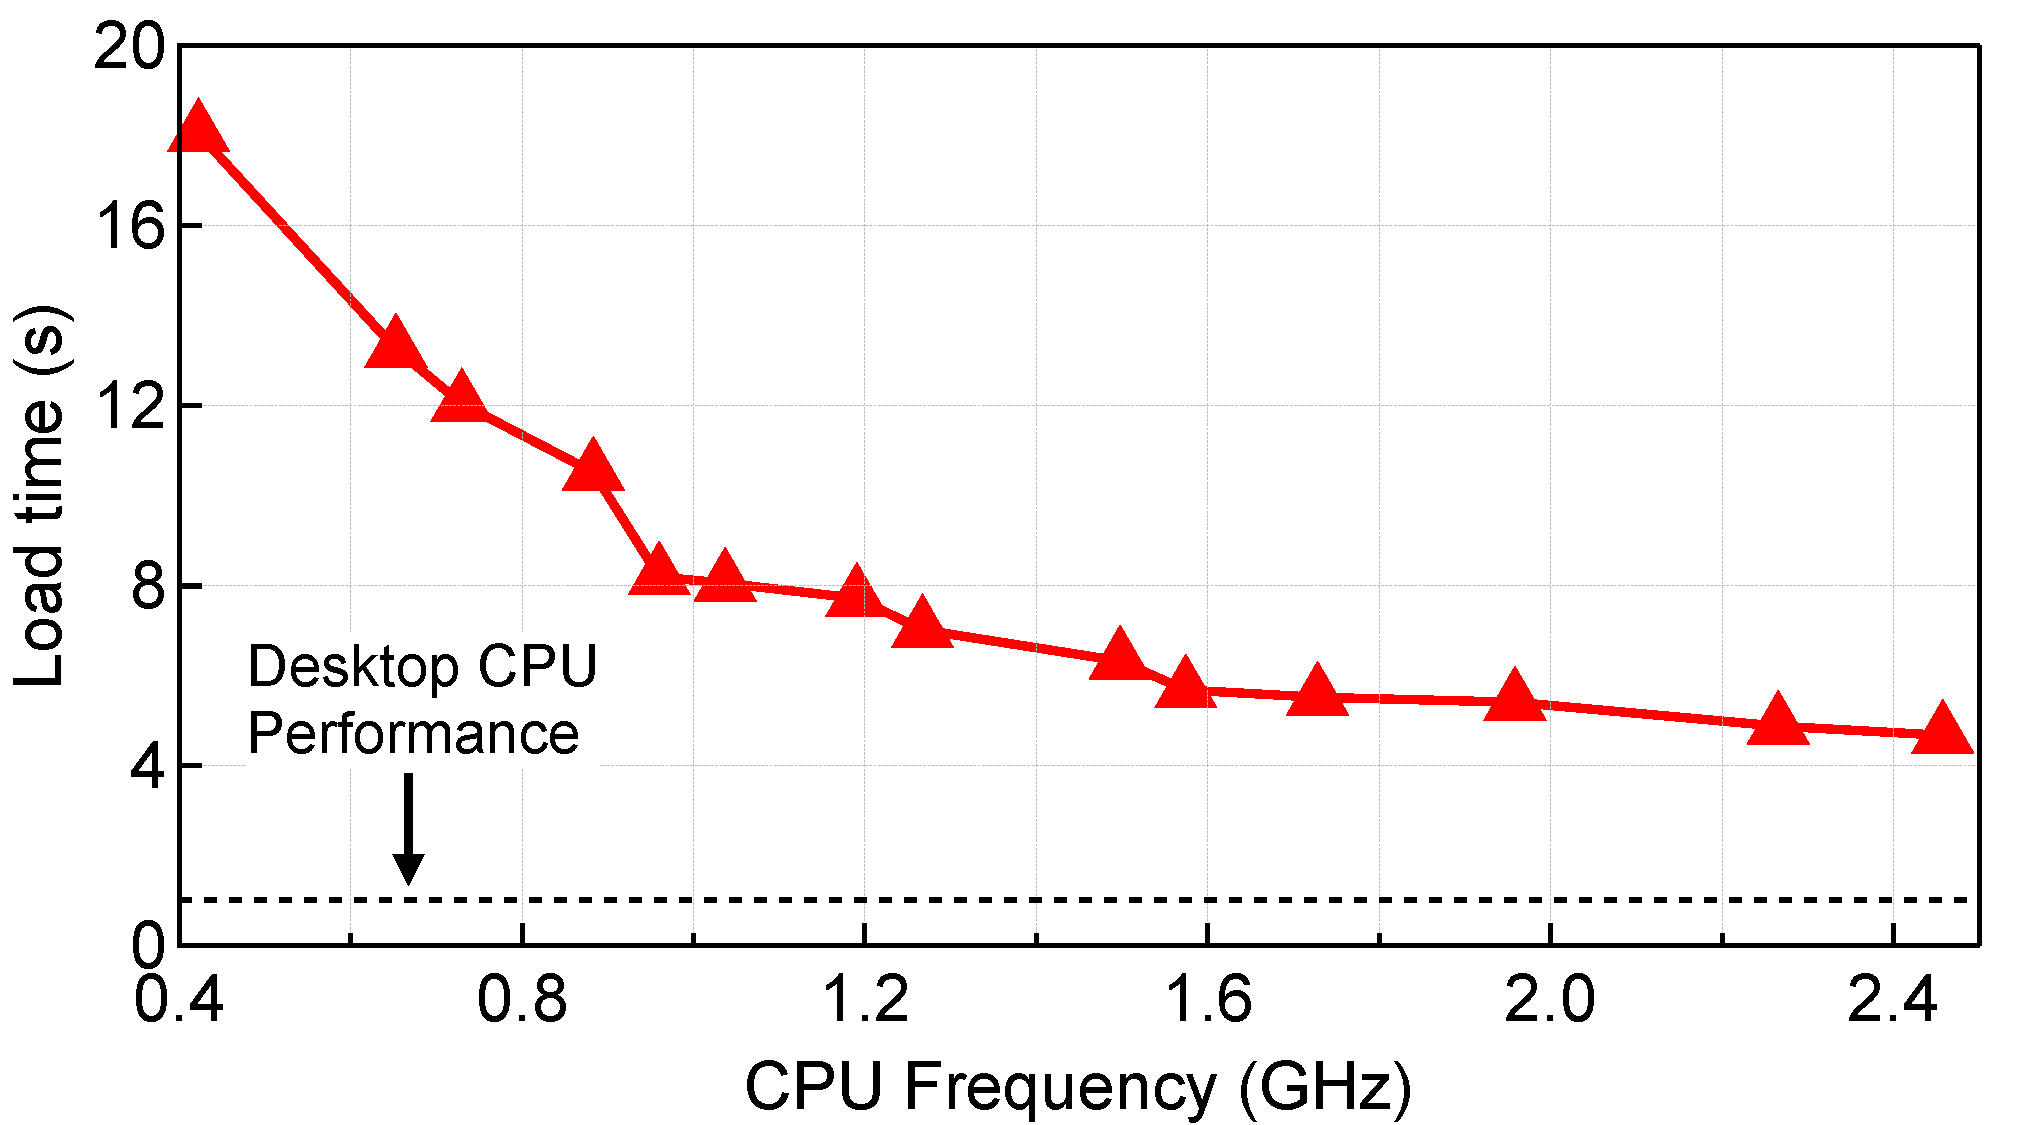
\includegraphics[trim=0 0 0 0, clip, width=.9\columnwidth]{cpu_bottleneck}
  \caption{Webpage load time with respect to CPU frequency on a Galaxy S5 smartphone. The markers represent CPU frequencies, which range from 0.4~GHz (left) to 2.5~GHz (right). We also overlay the load time on a desktop CPU (the dotted line) for comparison purpose.}
  \label{fig:cpu_bottleneck}
\end{figure}

Note that increasing clock frequency between 1.6~GHz and 2.4~GHz yields small performance benefits. One may then naively conclude that mobile CPU performance improvements provide marginal improvements in Web performance. However, the ``marginal improvement'' is merely an artifact of using frequency as a performance proxy. At high frequencies, the processor's pipeline is already saturated, and the memory and interconnection become the microarchitecture-level bottlenecks~\cite{clockvsipc}. To overcome this artificial constraint and assess the impact of future mobile CPU improvements, we perform the same experiment on a desktop CPU (Intel Core i5 at 1.2~GHz). The result is shown as the dotted line in \Fig{fig:cpu_bottleneck}. The average webpage load time on the desktop CPU is about 1~second, effectively a 4X speedup over the peak performance of S5. This experiment shows that mobile CPU performance today is still far from reaching a diminishing return point, and it can continue to have a significant impact on mobile Web performance.

The takeaway from the results is that continuous improvement to network latency will eventually, if not already, take us to a point where further Web performance improvement will be unattainable without improving CPU performance.  This is a timely conclusion, especially when low latency cellular network, such as LTE, is already prevalent today. It is estimated that LTE's subscription will reach 1.37 billion (one-fifth of the world population) by the end of 2015~\cite{lte_subscription}. Note, however, that we do \emph{not} claim that network latency is irrelevant. When the network deviates from an ideal low-latency condition, or in emerging markets where high-latency network accesses are prevalent~\cite{em}, mobile Web performance is indeed constrained by the network latency.

\section{The Need for Energy-Efficient Computation}
\label{sec:motivation:energy}

Despite the need for high-performance computation, mobile devices are severely limited by a battery-imposed energy budget, which in turn limits the achievable performance. In this section, I first use smartphones to quantitatively demonstrate that the energy budget of mobile devices is likely to stay stringently constrained in the near future. I then show that the CPU is becoming the worst power and energy consumer of a mobile device as compared to other components such as display and radio. There is clearly a need for energy-efficient computation in the mobile Web. Data presented here is adapted from the results of a related project~\cite{mobilecpu} that I collaborated on.

\paragraph{Energy Constraint} Battery technology has not experienced Moore's law-like improvements because of fundamental physics limitations~\cite{battery-mooreslaw}. As a result, the density of lithium-ion batteries has improved by only about 10\% per year~\cite{battery-stats}. Thus, the battery capacity of today's mobile devices is determined by the battery's volume, which is largely dictated by the device's screen size~\cite{phonescreen}. Using the smartphone as an example of a start-of-the-art mobile device, \Fig{fig:screen_batt} compares the screen sizes and battery capacities of over 600 smartphones from 2006 to 2014. There is a near-linear correlation between the battery capacity and screen size. As smartphone form factors reach maturity~\cite{phonesize}, the total device energy budget will likely stay severely constrained.

\begin{figure}[t]
  \centering
  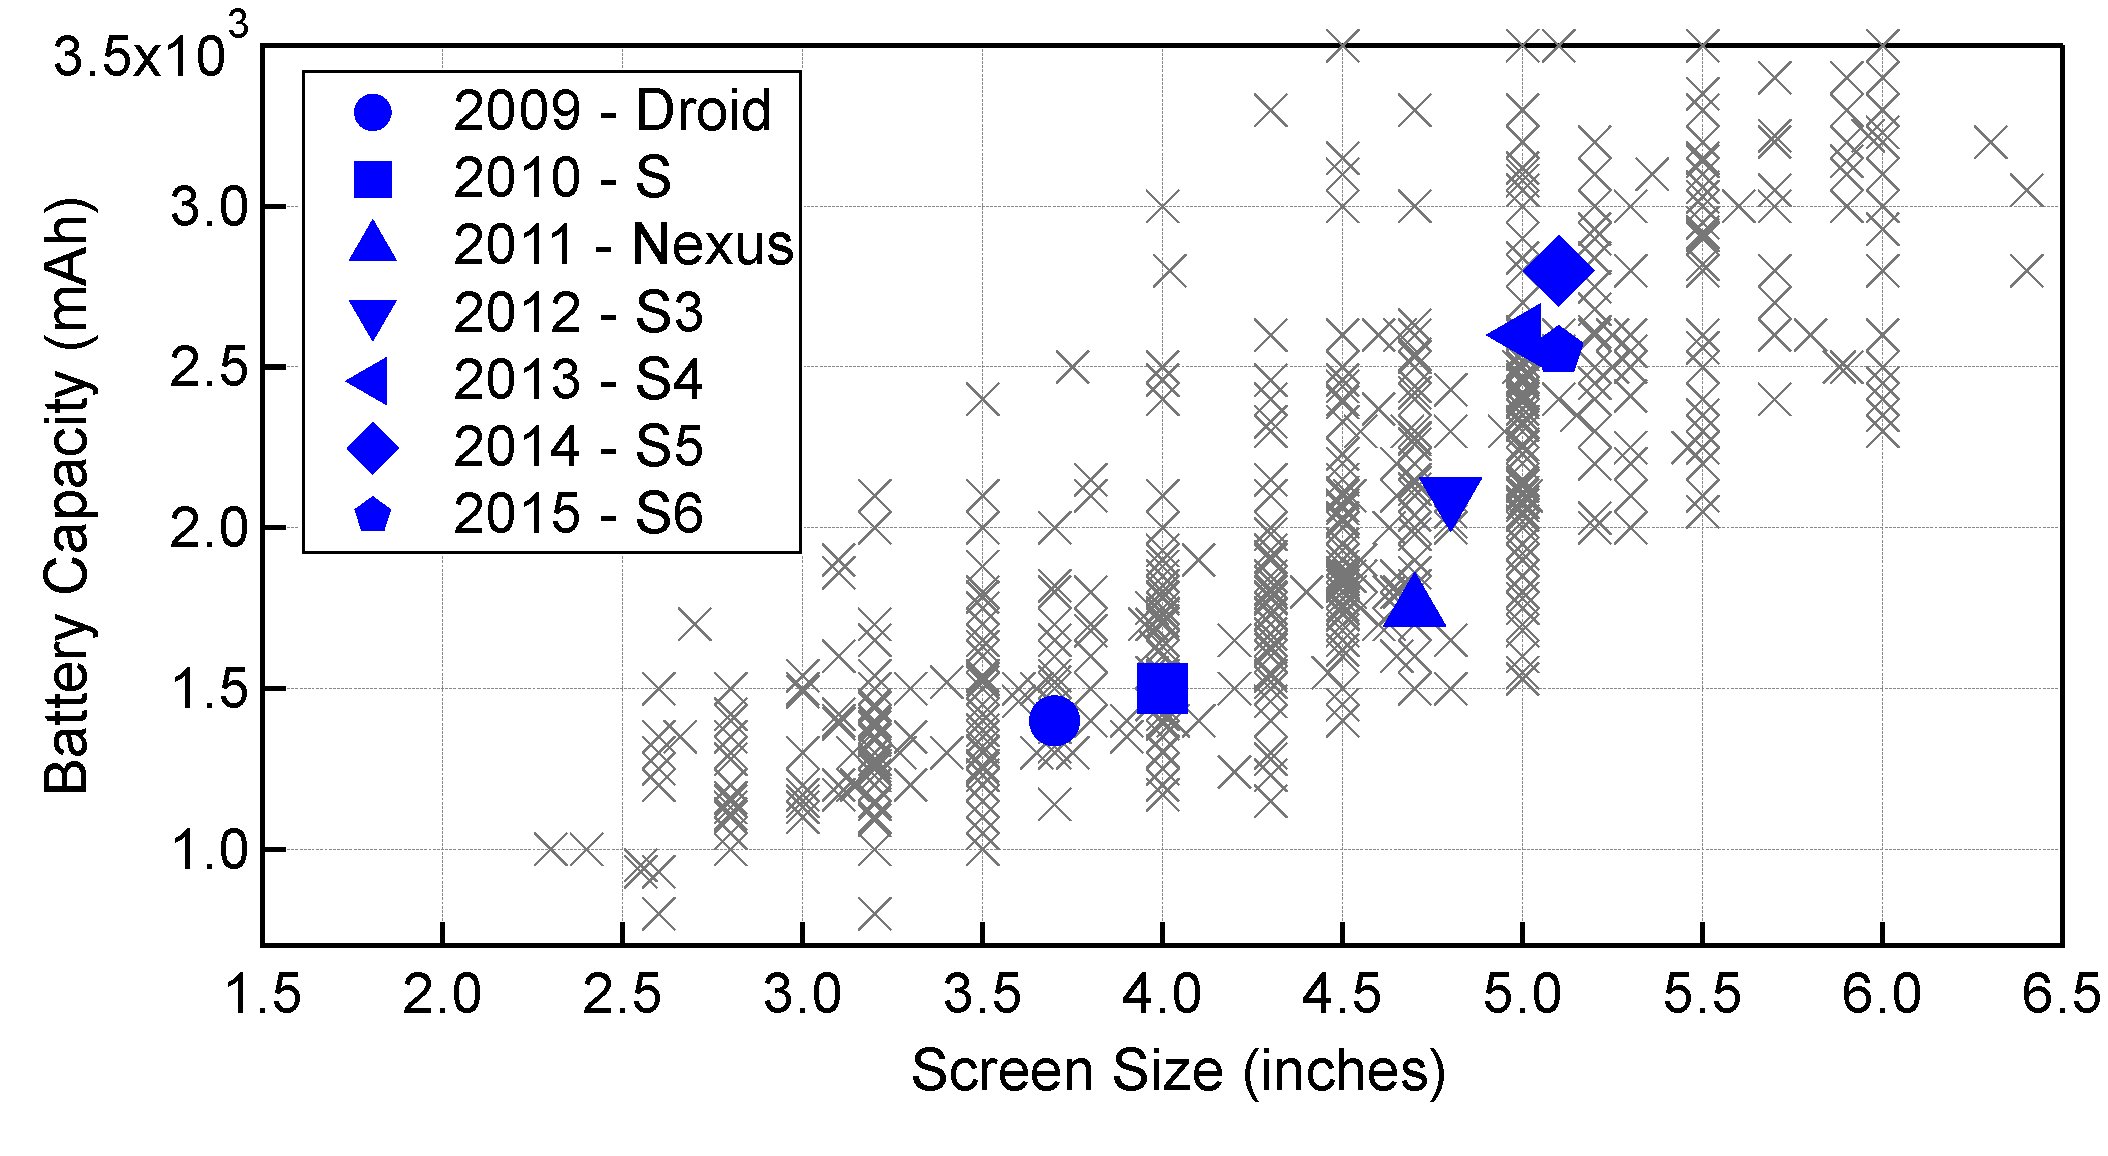
\includegraphics[trim=0 0 0 0, clip, width=.9\columnwidth]{screen_batt}
  \caption{The correlation between smartphone battery capacities and their screen sizes. There is an almost linear relationship over the time.}
  \label{fig:screen_batt}
\end{figure}

\begin{figure}[t]
  \centering
  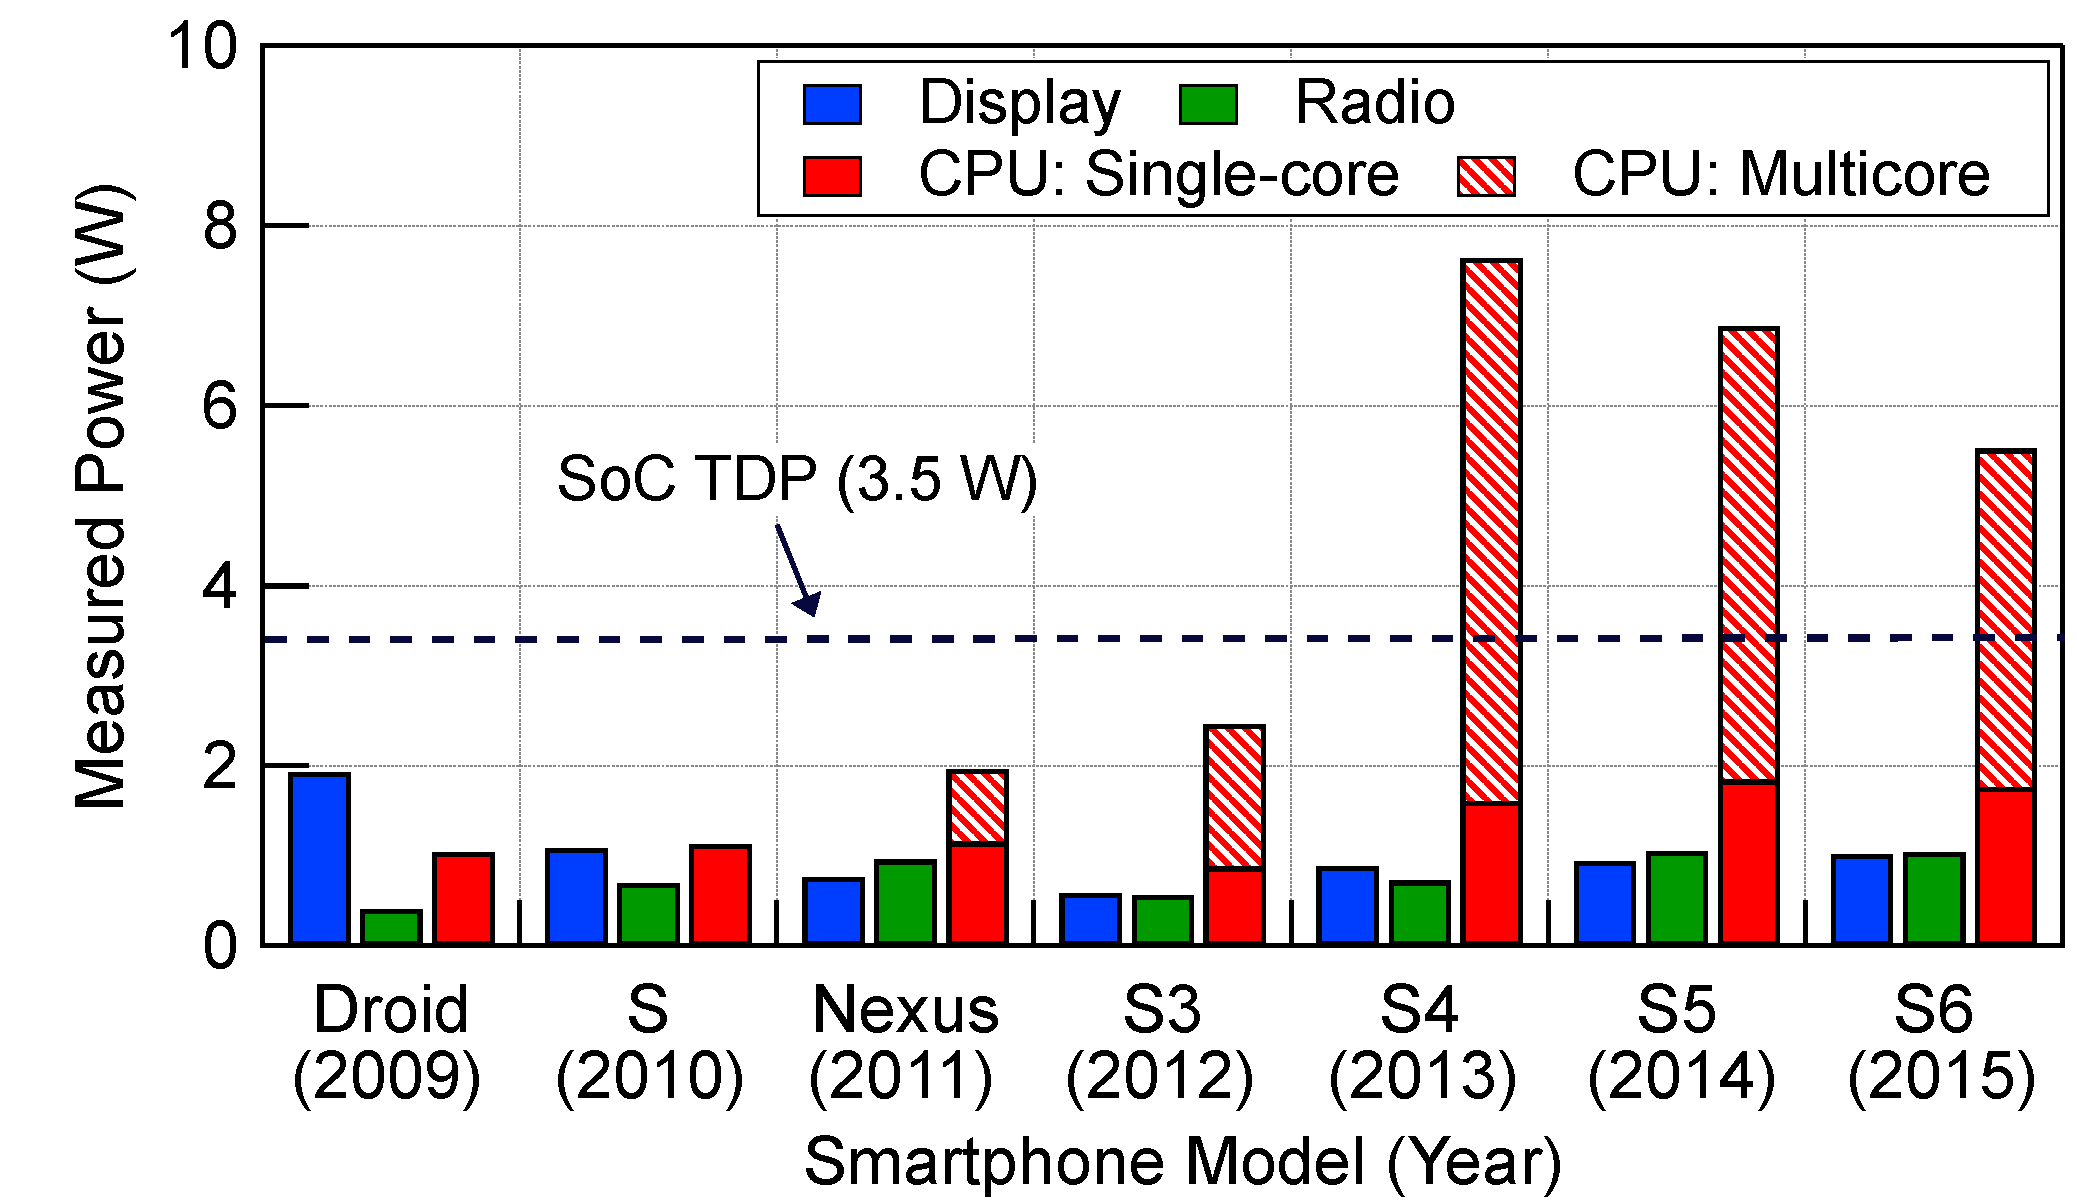
\includegraphics[trim=0 0 0 0, clip, width=.9\columnwidth]{phone_power_trend}
  \caption{CPU measured peak power consumption has increased significantly compared to other key mobile device components over the years. In particular, the multicore CPU power alone can exceed SoC-level TDP.}
  \label{fig:phone_power_trend}
\end{figure}

\paragraph{Mobile CPU's Rise to Power} Different components contribute to the overall power consumption of a mobile device. \Fig{fig:phone_power_trend} compares the measured power consumption of three major mobile device components: CPU, display, and radio. We select seven top smartphones for each year from 2009 to 2015. They are Motorola's Droid from 2009, and Samsung's Galaxy S, Nexus, S3, S4, S5, and S6 from 2010 through 2015, respectively. Chronologically, the seven phones represent how cutting-edge smartphone technologies have progressed over time. The results are collected while running a standard Web benchmark, Sunspider~\cite{sunspider}, for the CPU(s), and dedicated benchmarks for the other components~\cite{carroll2010analysis,ookla}. We used the Monsoon power monitor to measure the seven smartphones' power consumptions at the battery level.

We make two important observations from~\Fig{fig:phone_power_trend}. First of all, CPU has become a major power consumer in a mobile device. The year 2011 marks an inflection point where a single CPU core began overtaking the display as the most power consuming component. On any of the last three mobile CPU generations, the multicore CPU power consumption exceeds the entire mobile device's thermal design power~(TDP) even without considering the power consumption of radio, display, and the rest of the SoC.

Second, while other mobile device components are becoming more power-efficient over time due to their respective technological advancements~\cite{chen2013energy}, the CPU's power has risen excessively. The continuous mobile CPU power increase is a direct result of the mobile CPU design strategy, namely simply adopting desktop-like design techniques, such as aggressive single-core microarchitecture enhancement and multicore scaling, to improve performance at the expense of high power consumption. A recently study shows that mobile CPUs incorporated over 20 years of desktop CPU design techniques in just about seven years~\cite{mobilecpu}. The inevitable consequence of such a design methodology is that as the Dennard Scaling~\cite{dennard} comes to its end, the performance improvement can no longer make up for the additional power consumption~\cite{mobilecpu}, eventually making the mobile CPU extremely energy-inefficient.
%For example, I observed that the energy consumption improvement of Web browsing has already plateaued since 2012~\cite{zhu2015role}.
%A recent measurement study further suggests that the CPU contributes to about 50\% of the total device energy consumption for various mobile Web applications~\cite{mobilebench}.

Given that users expect each mobile device generation to incorporate new peripherals such as sensors that also require energy from the same budget, it is clear that the CPU, as a major energy consumer, needs to become more energy-efficient while sustaining performance improvement.














